%%%%%%%%%%%%%%%%%%%%%%%%%%%%%%%%%%%%%%%%%%%%%%%%%%%%%%%%%%%%%%%%%%%%%%
%
% Documento PRINCIPAL de Pedometria
% Newsletter da Sociedade Brasileira de Ciência do Solo
%
% Número 4, Julho de 2014
% 
% Language: Latex
% 
%%%%%%%%%%%%%%%%%%%%%%%%%%%%%%%%%%%%%%%%%%%%%%%%%%%%%%%%%%%%%%%%%%%%%%

% PREÂMBULO
\documentclass[a4paper]{report}

% Língua e codificação
\usepackage[brazilian]{babel}
\usepackage[utf8]{inputenc}
\usepackage[T1]{fontenc}
%\usepackage[latin1]{inputenc}
%\DeclareUnicodeCharacter{00A0}{~}

% para boot
\usepackage{amssymb,amsmath}

% Nota: é preciso incluir o pacote amsmath antes do pacote PEDOMETRIAnews
% porque o último redefine o ambiente de equações
\usepackage{PEDOMETRIAnews}
% Citações numéricas, usando sobrescritos, conforme usado em 'Nature'
% Referências para o pacote natbib: http://merkel.zoneo.net/Latex/natbib.php
\usepackage[numbers, super, sort&compress]{natbib}

% Figuras
\usepackage{graphicx}
\usepackage{float}
\usepackage{wrapfig}

% para Sweave
\usepackage{listings}
\usepackage{Sweave}

% cor para verbatim (ambiente para código fonte)
\usepackage{color}
\let\oldv\verbatim
\let\oldendv\endverbatim
\def\verbatim{\par\setbox0\vbox\bgroup\oldv}
\def\endverbatim{\oldendv\egroup\fboxsep0pt \noindent\colorbox[gray]{0.8}{\usebox0}\par}

% definição de \pedometria e \pedometriabf
\newcommand{\pedometria}{\textsc{PedometriA}}
\newcommand{\pedometriabf}{\textsc{\textbf{PedometriA}}}
\newcommand{\pedoartemetria}{\textbf{\sffamily Pedo[Arte]Metria}}
\newcommand{\pergunta}[1]{\vspace*{5mm}\noindent\pedometriabf{} - #1}
\newcommand{\resposta}[2]{\vspace*{5mm}\noindent\textbf{#1} - #2}

% definição de \PedoArteMetria
\newcommand{\PedoArteMetria}[4]{
  \noindent
  \begin{minipage}[t][0.95\textheight][t]{\textwidth}
    \textbf{\sffamily\Huge Pedo[Arte]Metria}\\
    \vspace*{0.5cm}\\
    \begin{figure}[H]
      \includegraphics[width=\textwidth]{#1}
    \end{figure}
    \vspace*{0.5cm}
    \raggedleft
    \begin{minipage}{0.8\textwidth}
      \raggedleft
      \LARGE
      \noindent\textbf{#2}\\
      \vspace*{0.5cm}
      \noindent{#3}
      \vspace*{0.5cm}\\
      \normalsize{\noindent\textit{Foto enviada por: #4}}
    \end{minipage}
    \vfill
    \raggedright
    \begin{minipage}{0.5\textwidth}
      \rule{\textwidth}{1mm}
      \normalsize
      Se você quer compartilhar conosco uma imagem \textbf{\sffamily Pedo[Arte]Métrica} de sua autoria, envie-a para \href{mailto:pedometria.news@gmail.com}{pedometria.news@gmail.com} com resolução de 300 dpi ou com no mínimo 5Mb, preferencialmente em formato PNG.
    \end{minipage}
  \end{minipage}
  }

% doi
\newcommand*{\doi}[1]{[\href{http://dx.doi.org/\detokenize{#1}}{link}]}
  
% para tcltk-update
\usepackage{shortvrb}
%\usepackage{chapterbib}

\sloppy{}

% links
\usepackage{hyperref} % Deve ser o último pacote carregado
\hypersetup{colorlinks=true, citecolor=blue, linkcolor=blue, urlcolor=blue}

% DOCUMENTO
\begin{document}
 
% Edição da newsletter
\volume{4}
\volnumber{4}
\date{Julho de 2014}
\titlepage
\begin{article}
   \title{Editorial}
\author{por Alessandro Samuel-Rosa}
\maketitle
\begin{wrapfigure}{l}{0.15\textwidth}
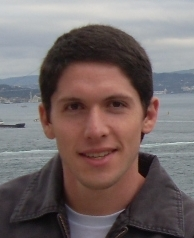
\includegraphics[width=0.15\textwidth]{figuras/foto-alessandro}
\end{wrapfigure}
O segundo número da \textit{Newsletter} da Comissão de Pedometria está cheio de novidades. A principal delas é a nova estrutura, muito mais bonita, graças à inestimável colaboração da comissão editorial do GRASS News, a newsletter do projeto \href{http://grass.osgeo.org/newsletter/}{GRASS}. Após contato com Martin Wegmann \email{wegmann@biozentrum.uni-wuerzburg.de}, editor-chefe do GRASS News, e Dylan Beaudette \email{debeaudette@ucdavis.edu}, administrador da página da web do GRASS News, formos gentilmente autorizados a usar o arquivo de estilo \texttt{GRASSnews.sty}, originalmente derivado do arquivo de estilo \texttt{Rnews.sty}, usado pela equipe do projeto \R{} para produção da sua newsletter. O agora arquivo de estilo da \textit{Newsletter} da Comissão de Pedometria da SBCS, \texttt{PEDOMETRIAnews.sty}, está disponível para baixar \href{http://goo.gl/OBWF3s}{clicando aqui}. É por meio do arquivo de estilo \texttt{PEDOMETRIAnews.sty} que a \textit{Newsletter} fica com a cara que ela tem hoje. Mais informações sobre o uso de \LaTeX{} para a produção de documentos técnico-científicos podem ser encontradas no site da \href{http://www.elsevier.com/author-schemas/preparing-documents-with-tex}{Elsevier}.\\
A evolução da \textit{Newsletter} em seu segundo número acompanha a evolução da pedometria no Brasil, claramente evidenciada pelo volume de trabalhos publicados no Congresso Brasileiro de Ciência do Solo (CBCS), em Florianópolis, há alguns meses atrás. Somam-se aí os espaços destinados mesas de discussão constituídas por importantes pesquisadores da pedometria nacional e internacional. O espaço destinado pela Comissão Organizadora do CBCS mostra que a comunidade científica nacional, assim como já ocorre há mais de uma década em outros países, está muito interessada nas contribuições da mais nova disciplina da ciência do solo. Uma disciplina que exige, como mostram os artigos que seguem, uma abordagem mais do que multidisciplinar ou interdisciplinar. Uma disciplina que exige uma abordagem \href{http://www.fisica-interessante.com/files/artigo-transdisciplinaridade.pdf}{transdisciplinar}, forçando-nos a transpor os limites das disciplinas tradicionais da ciência do solo e mergulhar em um universo de novas maneiras de 
encarar velhos problemas.
%%% Local Variables: 
%%% mode: latex
%%% TeX-master: documento-principal.tex
%%% End: 


\end{article}
\newpage
\PedoArteMetria{figuras/pedoartemetria}{A cor do solo}{Para um olhar desavisado, não se trata de maquiagem. São porta amostras para avaliação da espectroscopia de refletância difusa, uma das técnicas mais indicadas para quantificar os óxidos de ferro (hematita e gohetita) como alternativa a técnica convencional de difração de Raio-X.}{Diego Silva Siqueira -- Grupo de Pesquisa CSME da UNESP Campus de Jaboticabal}
\begin{article}
   \title{Projeto Biblioteca Espectral de Solos do Brasil - BESB}
\author{por José Alexandre M. Demattê e Marilusa P. C. Lacerda}
\maketitle

A população mundial compreende, atualmente, cerca de 7.207.456 bilhões de pessoas e é esperado um valor de 8.612.262 até 2050, segundo dados da \citet{FAO:2013}. Como alimentar essa população? Em 2006, na Conferência Mundial em Infra-estrutura Geospacial e banco de dados, ocorrida no Chile, com 63 países participantes, concluiu-se que para atender as necessidades da população mundial crescente nesta proporção, será necessária a elaboração de mapas temáticos dos recursos naturais em escalas detalhadas (entre eles solos), bem como a organização dos dados relacionados em bancos de dados digitais, como forma de subsidiar o planejamento das atividades agrícolas e produção de alimentos. Afora o lado da necessidade humana, destaca-se a importância do agronegócio no Brasil. Do valor bruto da produção do agronegócio brasileiro, que chegou a R\$470 bilhões em 2013, 66\% refere-se à agricultura. Somente a China, em 2013, comprou do Brasil US\$23 bilhões só em alimentos, e das exportações totais de soja nos próximos 10 anos, 71,3\% devem ser dirigidas para a China \citep{Brasil:2013}. Estes dados mostram a força do Brasil na agricultura e na economia mundial.\\
\\
\begin{figure}[htbp]
   \centering
   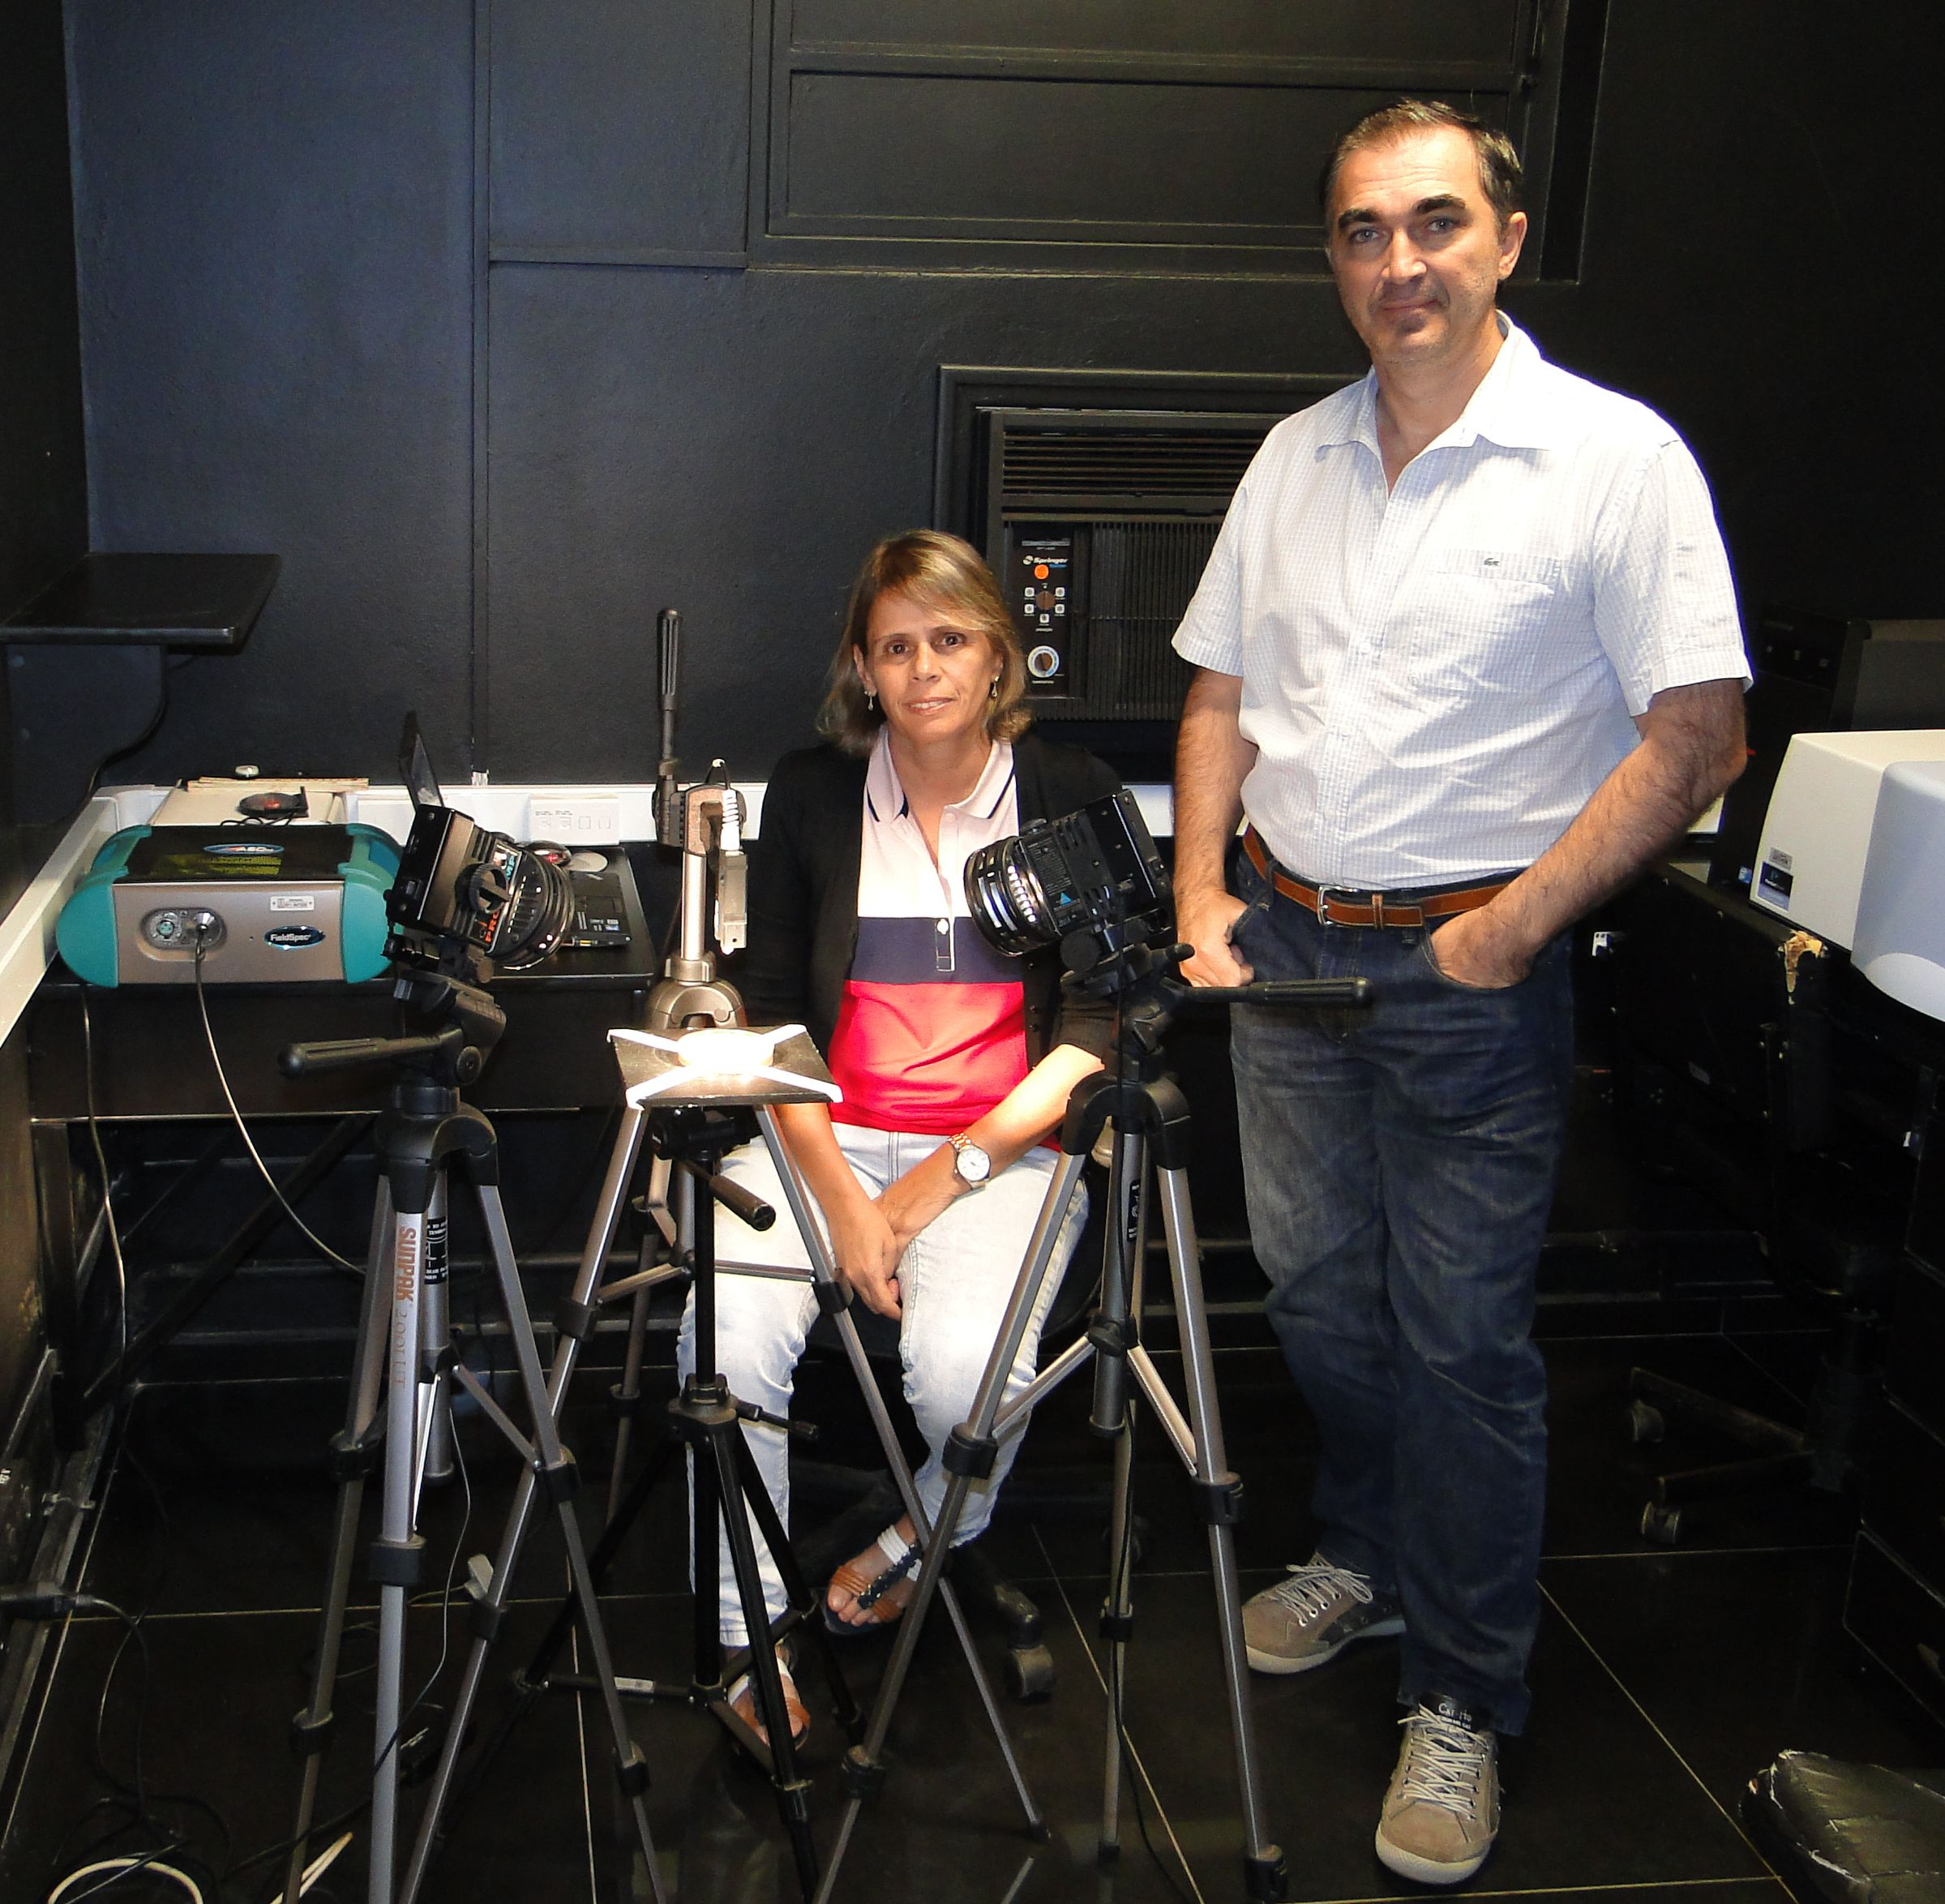
\includegraphics[width=0.8\textwidth]{figuras/dematte-marilusa.jpg}
   \caption{Os autores no Laboratório de Sensoriamento Remoto e Geoprocessamento Aplicado a Solos e Uso da Terra do Departamento de Ciência do Solo da Escola Superior de Agricultura Luiz de Queiroz.}
   \label{fig:autores}
\end{figure}

Por outro lado, apesar de precisarmos do solo, não o tratamos adequadamente. \citet{Mahmood:1987} já destacava a grande perda de solos pelas atividades antrópicas sem planejamento adequado, por intermédio do elevado acúmulo de sedimentos nos reservatórios de água do mundo. A maioria da literatura disponível mostra que o transporte anual de sedimentos, incluindo solos erodidos, para os oceanos pelos rios do mundo, é de 15-20 bilhões de Mg de acordo com \citet{Lal:2003}. O uso de herbicidas no solo varia de g a kg nos Estados Unidos e vários outros países desenvolvidos, causando sérios problemas aos solos e lençóis freáticos \citep{SinghEtAl:2010}. A ocorrência de CO$_2$ na atmosfera aumentou em 36\% entre 1750 e 2006 \citep{CoelhoEtAl:2013}, causado pelo uso inadequado dos solos. Os solos tem importância nos teores de carbono orgânico e inorgânico, que por sua vez tem relação com as questões atmosféricas e climáticas \citep{Lal:1999}.

\subsection*{Como evitar e solucionar estes problemas?}

Conhecer os solos, seus atributos e sua espacialidade estão intimamente relacionados ao apoio na resolução de vários dos problemas apontados. O conhecimento espacializado dos solos podem auxiliar em: conservação do solo, planejamento do uso da terra, alocação varietal, planejamento experimental, planejamento em manejo de solo (aração, gradagem, descompactação, entre outros), manejo dos ambientes (épocas de plantio, colheita), planejamento paisagístico, urbanos, na área de engenharia, entre inúmeras outras funções. Basta saber usar.

O Brasil teve grandes avanços em mapeamentos pedológicos realizados nas décadas de 70 e 80, mas a escala de pouco detalhamento utilizada permitiu somente avaliações estratégicas e não são adequados para o nível agrícola atual. Por outro lado, para a real importância destes mapas para a expansão da agricultura em grandes proporções são necessários mapas de solos em níveis detalhados em grandes escalas (faixa de 1:20.000). Neste quesito, estamos ``a pé'' e longe da real necessidade do país. Na realidade, o Brasil possui, no máximo, 0,25\% do seu território com mapas pedológicos detalhados ou semi-detalhados \citep{Mendonca-SantosEtAl:2007}.

\subsection*{O uso de Sensoriamento Remoto no mapeamento de solos em escalas detalhadas no Brasil}

Diante da grande extensão territorial do Brasil, falta de pessoal especializado e financiamentos de grande amplitude, somente com a agregação das geotecnologias aos métodos clássicos de levantamento e mapeamento de solos será possível atingir nosso intento. Dentre estas geotecnologias, ressalta-se o sensoriamento remoto (SR), definido basicamente como ``a aquisição de dados de um objeto sem haver contato direto com o mesmo''. Esse dado pode ser em diversos níveis de aquisição desde laboratorial, campo, aéreo e orbital. 

Para que tal tecnologia se desenvolva, é extremamente importante que entre na grade de ensino, em especial, na área de agronomia, as técnicas (dentro das quais entra o SR e o mapeamento digital) de mapeamento de solos e a sua aplicação no processo agrícola. O mapeamento é o resultado do estudo nas mais diversas áreas da ciência do solo, sendo a base no processo de planejamento agrícola. Logo, não há como fugir a inserção do aparato tecnológico na área de ensino, sob pena de perda do interesse dos alunos. Por outro lado, a base fundamental (Pedologia, gênese, trabalhos de campo) deve continuar a ser dada em consonância ao avanço tecnológico. 

A espectroscopia, metodologia associada ao SR, é uma ferramenta poderosa para a detecção e análise de alvos, baseada na interação da radiação eletromagnética (REM) com a matéria. A REM em comprimentos de onda diferentes transporta quantidades de energia diversificadas e proporcionam interações variadas entre as moléculas e os átomos que podem interagir com os fótons (ondas eletromagnéticas), absorvendo, transmitindo ou refletindo energia. A energia refletida pode ser medida por um equipamento específico, o espectrorradiômetro, definindo a espectroscopia de emissão, com medições da radiância ou reflectância da REM. O resultado é a obtenção de assinaturas ou curvas espectrais específicas de cada material analisado em vários intervalos de comprimento de onda do espectro eletromagnético, desde o Visível (400-750~nm), Infravermelho Próximo e Médio (750-2.500~nm) (Figura \ref{fig:curvas}), podendo atingir o Infravermelho Médio (2500-25000~nm). Basicamente, tal tecnologia pode e deve ser associada a metodologias matemáticas, estatísticas e geoestatísticas para atingir melhores resultados em pedotransferências. A espectroscopia se destaca por ser um procedimento rápido, não destrutivo, de menor custo e que, praticamente não proporciona impactos ambientais, quando comparado às metodologias tradicionais. Basicamente os dados espectroscópicos adquiridos têm duas funções: a) quantificar atributos de solos, tais como teores de argila, areia, Fe$_2$O$_3$, carbono orgânico, valores de Ki, CTC, entre outros \citep{Soriano-DislaEtAl:2014}; e b) a assinatura espectral de amostras dos horizontes de um perfil pedológico permite inferir a provável classe deste solo \citep{VasquesEtAl:2014}. Uma das grandes vantagens do método é que de uma única leitura e em um mesmo aparelho, pode-se diagnosticar inúmeras informações sobre o solo, como seus atributos e o padrão da curva espectral terá correlação com a provável classe de solo. Além disso, os dados espectroscópicos adquiridos em laboratório têm outros itens de importância tais como: base para o entendimento dos padrões espectrais obtidos no campo; base para a compreensão dos dados alcançados por sensores instalados em aviões e satélites; base para a compreensão dos recentes avanços de sensores hiperespectrais; meio de comunicação entre a comunidade científica (pois o espectro é igual para todos), entre outras.

\begin{figure*}[tb!]
\begin{minipage}[t]{1\linewidth}
   \centering
   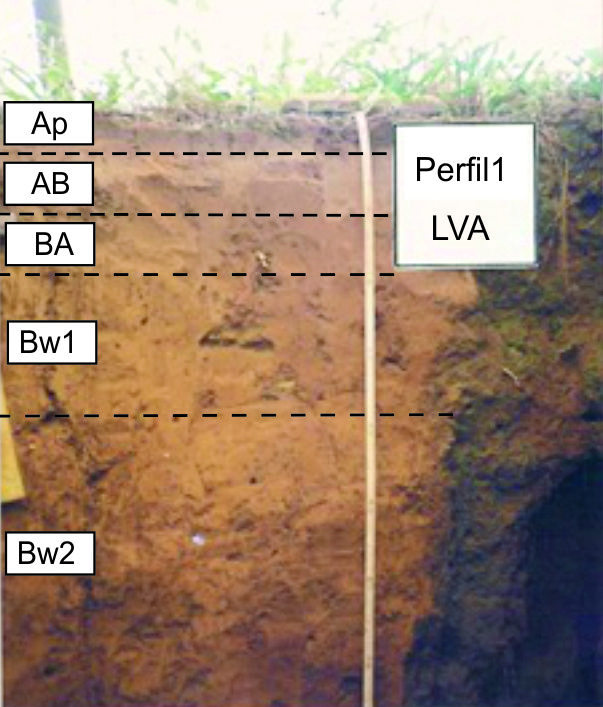
\includegraphics[width=0.49\textwidth]{figuras/lva.jpg}
   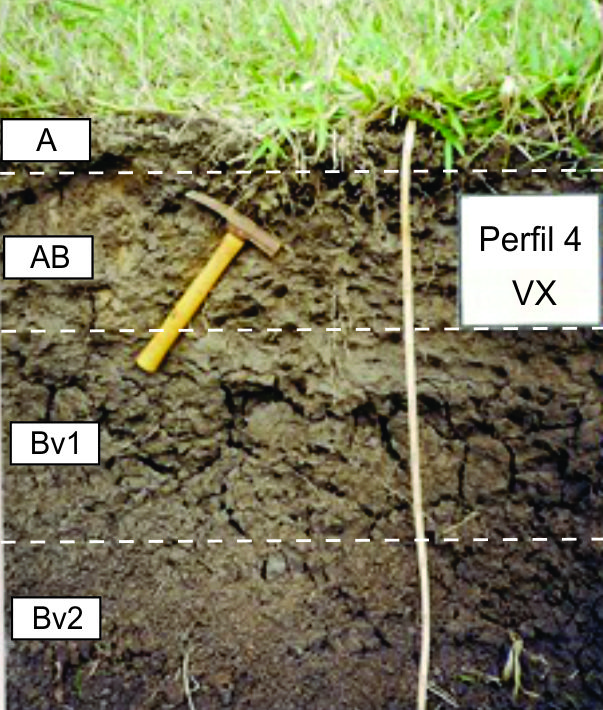
\includegraphics[width=0.49\textwidth]{figuras/vertissolo.jpg}
   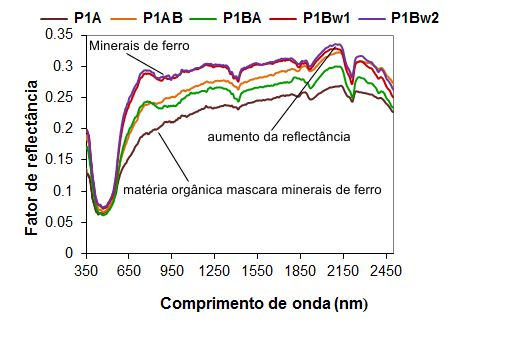
\includegraphics[width=0.49\textwidth, trim=0.5cm 0cm 1.5cm 0cm, clip]{figuras/curvas-lva.jpg}
   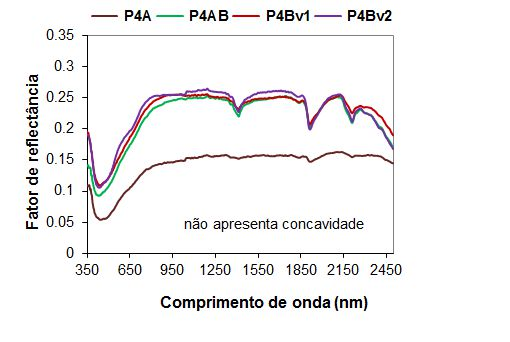
\includegraphics[width=0.49\textwidth, trim=0.5cm 0cm 1.5cm 0cm, clip]{figuras/curvas-vertissolo.jpg}
   \caption{Relações entre classes de solos e suas curvas espectrais. Solo 1 -- Latossolo Vermelho-Amarelo e curvas espectrais dos horizontes Ap, AB, BA, Bw1, Bw2. Solo 2 -- Vertissolo Háplico e curvas espectrais dos horizontes A, E, Bv1 e Bv2.}
   \label{fig:curvas}
\end{minipage}
\end{figure*}

\subsection*{Biblioteca Espectral de Solos do Brasil - BESB}

Um dos pilares para o sucesso de futuros mapeamentos de solos no Brasil é a montagem de bancos de dados de espectros de solos, aqui denominada Biblioteca Espectral de Solos do Brasil (BESB). Tal projeto trata da aquisição e armazenamento de padrões de curvas espectrais adquiridas de amostras de solos de várias regiões do Brasil. Tem por objetivos: (a) ter num único local, armazenadas informações relevantes de solos para estudos futuros; (b) realizar publicações iniciais demonstrando a utilidade desta poderosa ferramenta utilizando simultaneamente os dados de todo o Brasil; (c) estabelecer e consolidar uma comunidade que comece a entender e utilizar na prática a espectroscopia de solos; (d) ser a base para a comunidade pedológica em futuras pesquisas com adoção de novas tecnologias locais e regionais; (e) ser um pilar de apoio no mapeamento de solos; (f) ser um embasamento para o entendimento de dados obtidos por sensores aéreos e orbitais no território nacional.

Várias iniciativas têm sido realizadas no mundo desde \citet{StonerEtAl:1981}, até \citet{ShepherdEtAl:2002}, e \citet{BrownEtAl:2006}. No Brasil, o trabalho pioneiro foi de \citet{EpiphanioEtAl:1992}, publicado por \citet{FormaggioEtAl:1996} para o estado de São Paulo. Posteriormente, e com o objetivo de demonstrar a aplicação em mapeamento de solos, o primeiro trabalho realizado para cinco estados nacionais foi feito por \citet{BellinasoEtAl:2010}. A aplicação da técnica de sensoriamento remoto aplicada em mapeamento de solos foi descrita pela primeira vez no Brasil em 2004 por \citet{DematteEtAl:2004}, os quais seguiram a metodologia tradicional, porém aplicando os conceitos de espectroscopia. Em adição a isso, \citet{DematteEtAl:2001} já haviam associado a metodologia tradicional com fotos aéreas e espectroscopia, atingindo 90\% de coincidência com um trabalho realizado utilizando unicamente as técnicas tradicionais de levantamento e mapeamento de solos. Isso nos leva a outras aplicações de importância relevante nas Ciências Agrícolas, Ambientais e Agricultura de Precisão \citep{ThomassonEtAl:2001, OdlareEtAl:2005}. Na Europa, um grande projeto denominado \href{http://eusoils.jrc.ec.europa.eu/projects/Lucas/}{LUCAS} (Land Use/Cover Area frame Statistical Survey) foi elaborado na forma de banco de dados em 2013 com 20.000 amostras de solos recobrindo 23 países. Porém, o foco desta biblioteca está na quantificação dos solos e não classificação. Em contrapartida, outro projeto em andamento iniciado em 2008 compreende a participação de 80 países com a criação de um grupo em espectroscopia de solos, coordenado por \href{http://groups.google.com/group/soil-spectroscopy}{Viscarra Rossel}, relacionando as amostras de solos com classes e atributos dos mesmos \citep{ViscarraRossel:2009}.

Devido a tudo isso, foi proposta a primeira Biblioteca do Brasil, BESB (\url{http://bibliotecaespectral.wix.com/esalq}), cujas pesquisas estão sendo coordenadas pelo Prof. José Alexandre M. Demattê e pelo Grupo de Pesquisas em Geotecnologia em Ciência do Solo (\href{http://esalqgeocis.wix.com/geocis}{GeoCis}) no Laboratório de Sensoriamento Remoto e Geoprocessamento Aplicado a Solos e Uso da Terra do Departamento de Ciência do Solo da Escola Superior de Agricultura Luiz de Queiroz (ESALQ-USP) (Figura \ref{fig:autores}). Este projeto está vinculado ao já criado Grupo de Pesquisa em Espectroscopia de Solos do Brasil (GESB) pelo CNPq. Tal projeto atualmente conta com a colaboração de pesquisadores de dezenas de instituições parceiras, como a Empresa Brasileira de Pesquisa Agropecuária (Embrapa), o Instituto Agronômico de Campinas e diversas Universidades Estaduais e Federais, com representantes da Rede de Mapeamento Digital de Solos do Brasil (RedeMDS).

Até o momento, a Biblioteca Espectral de Solos do Brasil já reuniu informações de dez estados, com 14.839 amostras de solos já processadas e várias outras sendo preparadas para análises. Destas, 90\% pertencem ao acervo do Departamento de Ciência do Solo, oriundas de pesquisas diversas coordenadas pelo Prof. Demattê, sendo as demais cedidas por parceiros externos.

Atualmente, a Biblioteca está sendo desenvolvida por meio de aquisição de dados analíticos de atributos químicos básicos dos Solos (principalmente, matéria orgânica e/ou carbono, P, Ca, Mg, K, Al, H, pH, V\%, m\% e CTC), análises granulométricas (teores de areia, silte e argila) e curvas espectrais obtidas na faixa de comprimento de onda de 400-2500 nm por meio do equipamento denominado ASD Fieldspec. Para algumas amostras pretende-se obter dados em 2500-25.000~nm.

\subsection*{Como colaborar e utilizar a BESB?}

Toda a comunidade da Ciência do Solo do Brasil foi convidada a colaborar por meio de envio de amostras de solos de suas regiões. Para participar basta entrar no site da BESB e ver o protocolo. Resumidamente, os interessados devem: enviar amostras de perfis completos (com a designação dos horizontes), analises mínima química e granulométrica, classificação do solo e devem informar o local de coleta, preferencialmente com latitude e longitude (caso não seja possível, com o nome do município mais próximo). Como segunda opção, pode-se enviar amostras coletadas com trado, porém que se tenha, no mínimo, as camadas 0-20 e 80-100~cm no mesmo ponto, para que permita ter a variação analítica entre camadas. Informar a provável classificação do solo e demais informações da mesma forma que nos perfis. A quantidade de terra a ser enviada é de mínimo 50~g, secas, moídas e peneiradas (2~mm). Quem não tiver o equipamento, enviar para a ESALq que faremos as leituras e devolveremos os resultados. Se a instituição cedente tiver espectroradiômetro pode enviar diretamente as curvas espectrais para a ESALq, cujos resultados serão implementados no banco de dados, dentro do servidor do Laboratório de Sensoriamento Remoto e Geoprocessamento aplicado a Solos e Uso da Terra do Departamento de Ciência do Solo da ESALq-USP. O banco de dados já conta com amostras de estados como São Paulo, Goiás, Mato Grosso do Sul, Paraná, Minas Gerais, Rio Grande do Sul, Pernambuco, Pará, Mato Grosso e Amapá. Estão a caminho amostras da Amazônia, Distrito Federal, Rio de Janeiro, Tocantins, Maranhão, Santa Catarina e Acre (Figura \ref{fig:brasil}).

A equipe prevê a conclusão da BESB em etapas, sendo a primeira a ser concluída até o final de 2014 e a segunda em 2015. Os dados serão primeiramente publicados em estudos macro pela equipe organizadora. Num segundo passo, os dados serão disponibilizados aos respectivos responsáveis que cederam as informações, os quais poderão trabalhar nas escalas regionais, podendo estabelecer parcerias com qualquer membro participante da biblioteca (e que poderão ser localizados no site central) estabelecendo parcerias. Posteriormente, espera-se manter o sistema de maneira contínua. Os dados relativos a cada amostra estarão armazenados no banco de dados do servidor central, e serão disponibilizados sob autorização do pesquisador cedente. Cada um será o único responsável pelo seu dado e, portanto, terá autonomia sobre o mesmo. Os interessados em acessar as informações do acervo terão uma senha e buscarão os dados de acordo com a região de coleta das amostras. Também será possível, mediante autorização, usar dados de todo o território nacional ou de determinada região, para viabilizar estudos em parceria, de alcance macro e mostrando como é a distribuição de solos no país via assinatura espectral. A estratégia visa estreitar e fortalecer as relações entre diferentes grupos de pesquisa, favorecer a criação de novos polos e permitir que o fluxo de trabalho se autorregule em relação a futuras iniciativas derivadas do projeto.\\
\\
\begin{figure}
   \centering
   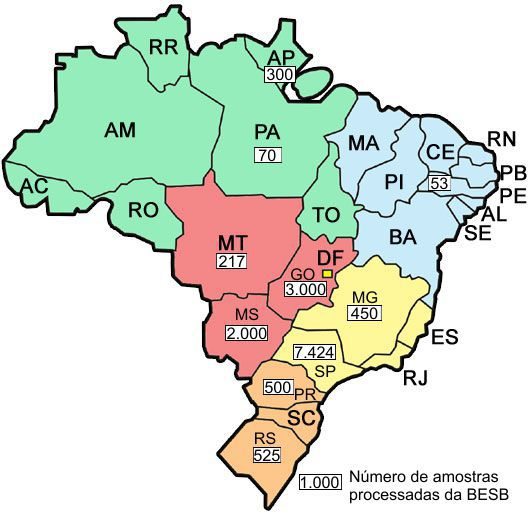
\includegraphics[width=0.8\textwidth]{figuras/brasil.jpg}
   \caption{Mapa do Brasil com a distribuição do número de amostras processadas por estado da Biblioteca Espectral de Solos do Brasil - BESB.}
   \label{fig:brasil}
\end{figure}

A biblioteca da ESALq armazena dezenas de artigos, dissertações e teses disponíveis em \url{http://esalqgeocis.wix.com/geocis}. Além disso, todos os dados gerais sobre o banco de dados e artigos específicos em espectrorradiometria encontram-se em \url{http://bibliotecaespectral.wix.com/esalq}.

\begin{footnotesize}
\begin{thebibliography}{99}

\bibitem[FAO(2013) FAO]{FAO:2013}
FAO (2013)
\newblock {\em State of the Art Report on Global and Regional Soil Information: Where are we? Where to go?}
\newblock Rome: FAO.

\bibitem[Brasil(2013) Brasil]{Brasil:2013}
Brasil (2013)
\newblock {\em Projeções do Agronegócio: Brasil 2012/2013 a 2022/2023.}
\newblock Disponível em \url{http://www.agricultura.gov.br/arq\_editor/projecoes\%20-\%20versao\%20atualizada.pdf}.

\bibitem[Mahmood(1987) Mahmood]{Mahmood:1987}
K. Mahmood (1987)
\newblock {\em Reservoir sedimentation - impact, extent and mitigation.}
\newblock Washington: World Bank.

\bibitem[Lal(2003) Lal]{Lal:2003}
R. Lal (2003)
\newblock Soil erosion and the global carbon budget.
\newblock {\em Environment International}, 29:437-450.

\bibitem[Singh \& Ghoshal(2010) Singh, Ghoshal]{SinghEtAl:2010}
P. Singh, N. Ghoshal (2010)
\newblock Variation in total biological productivity and soil microbial biomass in rainfed agroecosystems. Impact of application of herbicide and soil amendments.
\newblock {\em Agric. Ecosyst. Environ}, 137:241-250.

\bibitem[Coelho et~al.(2013) Coelho, Barbalho, Escremin]{CoelhoEtAl:2013}
A. Coelho, E.S. Barbalho, J.V. Escremin (2013)
\newblock Desenvolvimento de um experimento sobre o efeito estufa: uma proposta para o ensino.
\newblock {\em Rev. Virtual Quim}, 6:142-151.

\bibitem[Lal(1999) Lal]{Lal:1999}
R. Lal (1999)
\newblock {\em Métodos para a avaliação do uso sustentável dos recursos solo e água nos trópicos.}
\newblock Jaguariúna: Embrapa Meio Ambiente.

\bibitem[Mendonça-Santos \& Santos(2007) Mendonça-Santos, Santos]{Mendonca-SantosEtAl:2007}
M.L. Mendonça-Santos, H.G. Santos (2007)
\newblock The state of the art of brazilian soil mapping and prospects for digital soil mapping.
\newblock {\em Developments in soil science}, 31:39-54.

\bibitem[Soriano-Disla et~al.(2014) Soriano-Disla, Janik, Viscarra Rossel, Mac Donald, McLaughlin]{Soriano-DislaEtAl:2014}
J.M. Soriano-Disla, L.J. Janik, R.A. Viscarra Rossel, L.M. Mac Donald, M.J. McLaughlin (2014)
\newblock The performance of visible, near-, and mid-infrared reflectance spectroscopy for prediction of soil physical, chemical, and biological properties.
\newblock {\em Applied Spectroscopy Reviews}, 49:139-186.

\bibitem[Vasques et~al.(2014) Vasques, Demattê, Ramirez Lopes, Terra]{VasquesEtAl:2014}
G.M. Vasques, J.A.M. Demattê, L. Ramirez Lopes, F.S. Terra (2014)
\newblock Soil classification using visible/near-infrared diffuse reflectance spectra from multiple depths.
\newblock {\em Geoderma}, \textit{in press}.

\bibitem[Stoner \& Baumgardner(1981) Stoner, Baumgardner]{StonerEtAl:1981}
E.R. Stoner, M.F. Baumgardner (1981)
\newblock Characteristic variations in reflectance of surface soils.
\newblock {\em Soil Sci. Soc. Amer. J.}, 45:1161-1165.

\bibitem[Shepherd \& Walsh(2002) Shepherd, Walsh]{ShepherdEtAl:2002}
K.D. Shepherd, M.G. Walsh (2002)
Development of reflectance spectral libraries for characterization of soil properties. Soil Science Society of America Journal, v.66, p.988-998.

\bibitem[Brown et~al.(2006) Brown, Shepherd, Walsh, Mays, Reinsch]{BrownEtAl:2006}
D.J. Brown, K.D. Shepherd, M.G. Walsh, M.D. Mays, T.G. Reinsch (2006)
\newblock Global soil characterization with VNIR diffuse reflectance spectroscopy.
\newblock {\em Geoderma}, 132:273-290.

\bibitem[Epiphânio et~al.(1992) Epiphânio, Formaggio, Valeriano, Oliveira]{EpiphanioEtAl:1992}
J.C.N. Epiphânio, A.R. Formaggio, M.M. Valeriano, J.B. Oliveira (1992)
\newblock {\em Comportamento espectral de solos do Estado de São Paulo.}
\newblock José dos Campos: INPE.

\bibitem[Formaggio et~al.(1996) Formaggio, Epiphanio, Valeriano, Oliveira]{FormaggioEtAl:1996}
A.R. Formaggio, J.C.N. Epiphanio, M.M. Valeriano, J.B. Oliveira (1996)
\newblock Comportamento espectral (4502.450 nm) de solos tropicais de São Paulo.
\newblock {\em Revista Brasileira de Ciência do Solo}, 20:467-474.

\bibitem[Bellinaso et~al.(2010) Bellinaso, Dematte, Romeiro]{BellinasoEtAl:2010}
H. Bellinaso, J.A.M. Dematte, S.A. Romeiro (2010)
\newblock Soil spectral library and its use in soil classification.
\newblock {\em R. Bras. Ci. Solo}, 34:861-870.

\bibitem[Demattê et~al.(2004) Demattê, Campos, Alves, Fiorio, Nanni]{DematteEtAl:2004}
J.A.M. Demattê, R.C. Campos, M.C. Alves, P.R. Fiorio, M.R. Nanni (2004)
\newblock Visible-NIR reflectance: a new approach on soil evaluation.
\newblock {\em Geoderma}, 121:95-112.

\bibitem[Demattê et~al.(2001) Demattê, Demattê, Camargo, Fiorio, Nanni]{DematteEtAl:2001}
J.A.M. Demattê, J.L.I. Demattê, W.P. Camargo, P.R. Fiorio, M.R. Nanni (2001)
\newblock Remote sensing in the recognition and mapping of tropical soils developed on topographic sequences.
\newblock {\em Mapping Sciences and Remote Sensing}, 38:79-102.

\bibitem[Odlare et~al.(2005) Odlare, Svensson, Pell]{OdlareEtAl:2005}
M. Odlare, K. Svensson, M. Pell (2005)
\newblock Near intrared reflectance spestrocopy for assessement of spatial soil variation in an agricultural field.
\newblock {\em Geoderam}, 126:193-202.

\bibitem[Thomasson et~al.(2001) Thomasson, Sui, Cox, Al-Rajehy]{ThomassonEtAl:2001}
J.A. Thomasson, R. Sui, M.S. Cox, A. Al-Rajehy (2001)
\newblock Soil reflectance sensing for determining soil properties in precision agriculture.
\newblock {\em Trans. Am. Soc. Agron. Eng.}, 44:1445-1453.

\bibitem[Viscarra Rossel(2009) Viscarra Rossel]{ViscarraRossel:2009}
R.A. Viscarra Rossel (2009)
\newblock The Soil Spectroscopy Group and the development of a global soil spectral library.
\newblock {\em EGU General Assembly Conference Abstracts}, 11:14021.

\end{thebibliography}
\end{footnotesize}

\address{José Alexandre M. Demattê\\
  Departamento de Ciência do Solo, ESALQ/USP\\
  \email{jamdemat@usp.br}}
  
\address{Marilusa P. C. Lacerda\\
  Faculdade de Agronomia e Medicina Veterinária, FAV/UnB\\
  \email{marilusa@unb.br}}
%%% Local Variables: 
%%% mode: latex
%%% TeX-master: 4th-edition.tex
%%% End: 
\end{article}
\newpage
\begin{article}
   \title{Ciência do solo sem fronteiras}
\author{por Yuri A. Gelsleichter}
\maketitle

\begin{wrapfigure}{l}{0.15\textwidth}
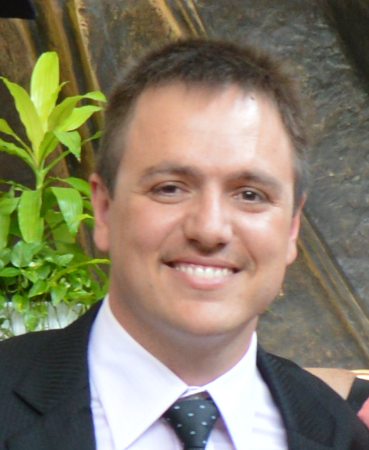
\includegraphics[width=0.15\textwidth]{figuras/yuri-foto}
\end{wrapfigure}

Olá amigo leitor, sou estudante de Engenharia Ambiental e Sanitária da Universidade do Sul de Santa Catarina (\href{http://www.unisul.br/wps/portal/home/}{UNISUL}), intercambista na Hungria, e gostaria de compartilhar com você um pouco de minha experiência no programa Ciência sem Fronteiras (\href{http://www.cienciasemfronteiras.gov.br/web/csf}{CsF}).

Essa história começou no meu ensino médio, após receber em minha turma um aluno vindo da Nova Zelândia. Desde então, tive o interesse de fazer intercâmbio, porém, sempre foi um sonho distante por diversos fatores: dinheiro, família, trabalho, namorada, comodidade, enfim, muitas coisas me prendiam, não sabia se em algum dia, poderia realizar isso, pensei até em morar no estrangeiro por conta própria com intuito do domínio de um segundo idioma e algumas aventuras. Mais recentemente imaginava que talvez o sonho fosse ser realizado através de um programa de mestrado ou doutorado no exterior.

Um dia no caminho para universidade escutando \href{http://conteudo.ebcservicos.com.br/programas/a-voz-do-brasil}{A Voz do Brasil}, ouvi o anúncio que seria lançado o programa de bolsas de estudo no exterior, financiado pelo governo federal. Desde o primeiro edital de CsF em 2011 comecei a me inscrever. Como muitos brasileiros tive a barreira do inglês, mas em nenhuma desisti, fui atrás fiz cursos e provas de inglês. E somente na quarta tentativa de participar do programa, a um semestre de me graduar, consegui a grandiosa oportunidade de fazer intercâmbio na modalidade de graduação sanduíche. Hungria foi meu destino. Largamos toda estabilidade adquirida, eu e minha devota esposa, e partimos sem olhar para trás.\\
\\
\begin{figure}[htbp]
   \centering
   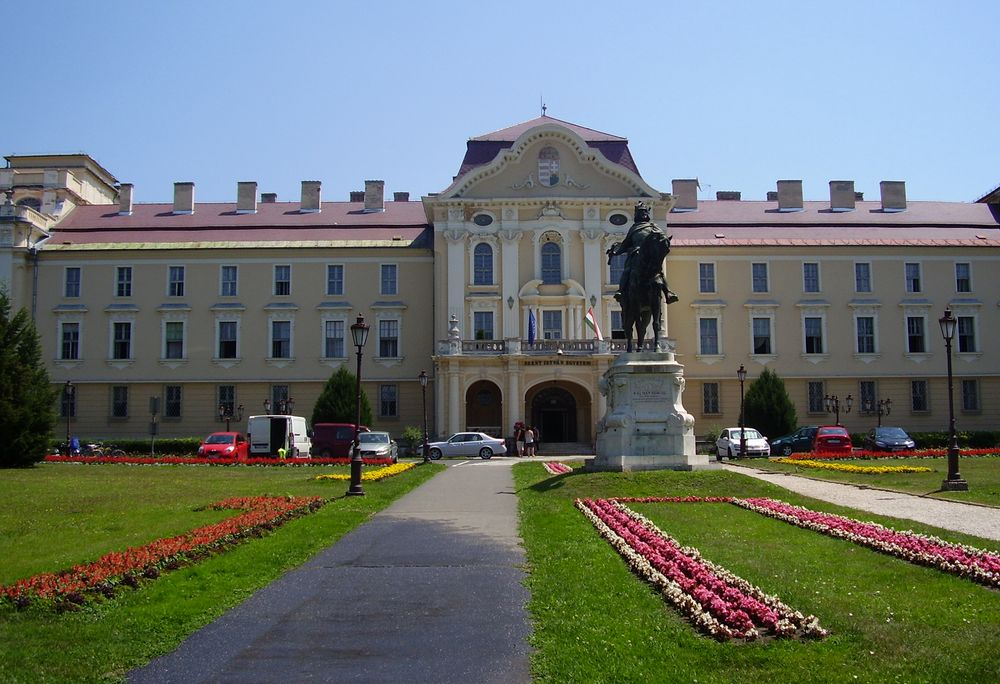
\includegraphics[scale=0.8]{figuras/yuri-foto-5}
   \caption{Prédio principal da Universidade Szent István. Fonte: \href{http://en.wikipedia.org/wiki/G\%C3\%B6d\%C3\%B6ll\%C5\%91}{Wikipédia}.}
   \label{fig:rótulo-da-figura}
\end{figure}
   
Tinha apenas um inglês básico e fui para o curso de dois meses, oferecido pelo programa na Hungria. Chegando ao destino em \href{http://en.wikipedia.org/wiki/G\%C3\%B6d\%C3\%B6ll\%C5\%91}{Gödöllő} na \href{http://sziu.hu/}{Universidade Szent István}, tudo era muito novo a cultura, o idioma, as pessoas, e me perguntava: como serão essas aulas em inglês, será que vou consegui acompanhar? Muitas dúvidas surgiram, mas após o curso intensivo e mais alguns dias de aula senti-me seguro e pronto.

\subsection{Ciência do solo sem fronteiras na Hungria}

No Brasil não tinha uma relação muito próxima dos estudos dos solos, mas gostei de estudar geologia e pedogênese. Na Hungria foram-me ofertadas disciplinas relacionadas ao estudo e conservação dos solos dentre outras. Logo nas primeiras aulas de solos com a professora \href{https://www.linkedin.com/profile/view?id=40499203&authType=NAME_SEARCH&authToken=tTwr&locale=en_US&srchid=1909093141405346286275&srchindex=1&srchtotal=1&trk=vsrp_people_res_name&trkInfo=VSRPsearchId\%3A1909093141405346286275\%2CVSRPtargetId\%3A40499203\%2CVSRPcmpt\%3Aprimary}{Dr. Michelí Erika} e sua equipe muito experientes, desde então tive grande interesse nos estudos dos solos. Intensivamente aprendi o funcionamento do sistema internacional de classificação de solos World Reference Base for Soil Resources (\href{http://www.fao.org/soils-portal/soil-survey/soil-classification/world-reference-base/en/}{WRB}), e paralelamente fui adentrando ao estudo das ciências dos solos e seus processos e características.\\
\\
\begin{figure}[htbp]
   \centering
   \includegraphics[scale=0.8]{figuras/yuri-foto-2}
   \caption{Saída de campo do semestre atual na disciplina \textit{Soil Degradation and Conservation}, envolvendo análise de solo e alteração geológica. Fonte: Arquivo pessoal.}
   \label{fig:rótulo-da-figura}
\end{figure}

Durante as disciplinas cursadas na Szent István tivemos muitas saídas de campo as quais possibilitaram um conhecimento mais direto e palpável, relacionadas principalmente, com o entendimento dos solos.

\subsection{Minha contribuicão ao Brasil}

No edital ao qual estou inserido foi previsto um estágio de trabalho e ou pesquisa. Não era tarefa fácil para a universidade alocar todos os alunos em atividades. Assim, estava aberto para os alunos escolherem suas atividades. Durante as aulas de solos foi utilizado como guia de estudo o WRB 2006. Ao ler no capítulo primeiro, que o texto principal está traduzido para 13 idiomas (chinês, francês, alemão, húngaro, italiano, japonês, letão, lituano, polonês, romeno, russo, espanhol e vietnamês), sugeri a tradução para o português, já que WRB é uma ``linguagem'' internacional e comum de solos, adotada oficialmente na Europa, Africa central e oeste, em outros países, como por exemplo: Itália, México, Noruega, Polônia e Vietnã. As atividades de tradução iniciaram-se após o fim do período de avaliações do primeiro semestre.\\
\\
\begin{figure}[htbp]
   \centering
   \includegraphics[scale=0.8]{figuras/yuri-foto-3}
   \caption{Análise de perfil de solo afetado por sal em saída de campo da  disciplina \textit{Soil Degradation and Conservation}. Fonte: Arquivo pessoal.}
\end{figure}

Segundo a Dr. Érika, que coordena o CsF na Szent István, com o programa houve uma grande troca de informações com o Brasil relacionadas aos dados de solos. Posteriormente houve a liberação do banco de dados dos perfis de solos brasileiros pela Embrapa. Durante o segundo semestre, após congresso mundial de solos na Coreia do Sul, fui convidado pela professora Dr. Érika a participar de um projeto para padronização e homogeneização do banco de dados de solos brasileiros, bem como sua ``tradução para o WRB e Soil Taxonomy US. Esse projeto tem a finalidade de dispor os dados para pesquisa a nível mundial, bem como o mapeamento mundial de solos.\\
\\
\begin{figure}[htbp]
   \centering
   \includegraphics[scale=0.8]{figuras/yuri-foto-1}
   \caption{Saída de campo semestre passado na  disciplina \textit{Modern Soil Observation and Conservation Methods}, com análise de perfis de solo em campo agrícola ao lado do campus da universidade. Fonte: Arquivo pessoal.}
\end{figure}

Segundo a Dr. Érika, também poderemos ser peças chaves no próximo congresso mundial de solos que será sediado no Brasil, devido ao fato do domínio da língua Inglesa e da ``linguagem'' internacional de solos, ou seja, dos nomes e termos técnicos na língua inglesa.

Concluindo, digo que em todos os locais que visitei e conheci pude perceber diferenças em relação ao Brasil, positivas e negativas. Penso que todos os estudantes de intercâmbio trazem dentro de si esses pontos positivos e naturalmente isso tende a gerar bons frutos para a sociedade brasileira tanto na academia como na cidadania.

\address{Yuri A. Gelsleichter\\
  Universidade do Sul de Santa Catarina\\
  \email{yuriplanta@gmail.com}}
%%% Local Variables:
%%% mode: latex
%%% TeX-master: 4th-edition.tex
%%% End:
\end{article}
\newpage
\begin{article}
   \title{Entrevista}
\subtitle{com Paulo Ivonir Gubiani}
\maketitle
\begin{wrapfigure}{l}{0.15\textwidth}
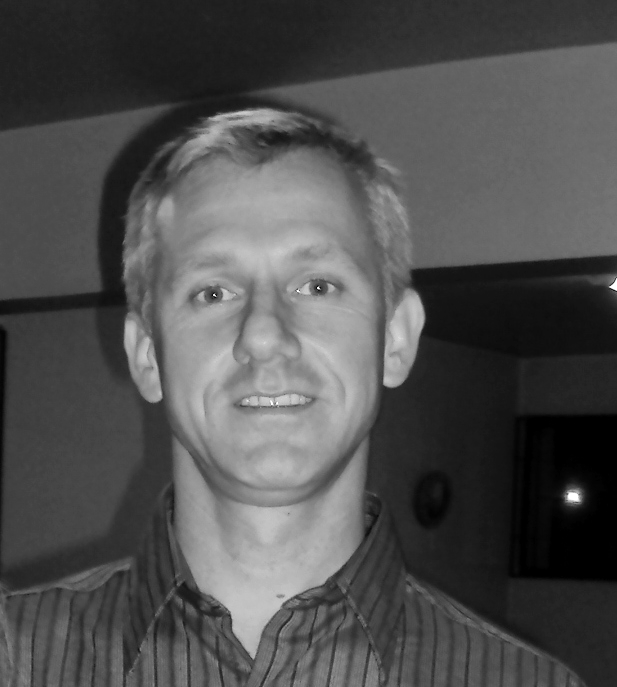
\includegraphics[width=0.15\textwidth]{figuras/foto-paulo}
\end{wrapfigure}

Nesta edição da \pedometria, entrevistamos o Professor Doutor Paulo Ivonir Gubiani para falar um pouco sobre sua experiência em modelagem matemática na área de Física do Solo, sua opinião com relação as pesquisas na área de modelagem, dificuldades e perspectivas futuras no Brasil. O Dr. Paulo atualmente é docente no Departamento de Solos - Setor de Física do Solo da Universidade Federal de Santa Maria (UFSM). Sua formação pós ensino médio foi realizada na UFSM, onde cursou Agronomia. Na mesma universidade fez seu mestrado e doutorado em Ciência do Solo na área de Processos Físicos e Morfogenéticos do Solo.

\pergunta{O que levou você a se interessar e estudar temas relacionados à modelagem matemática de dados ambientais, em especial, processos relacionados ao solo?}

\resposta{Paulo}{Penso que o estudo sobre modelagem matemática na área que atuo, isto é, Física do Solo, não é uma questão apenas de gosto ou interesse, mas sim de necessidade. O solo é um sistema aberto e dinâmico, e medidas pontuais de suas propriedades informam apenas estados do sistema. Na ciência, a medição constitui uma etapa fundamental, que é a observação. Porém, o ``fazer'' ciência vai muito além da observação. Em sistemas abertos e dinâmicos o principal interesse e função do pesquisador é conhecer a evolução do sistema no tempo, suas causas e consequências. As medições conseguem descrever o estado do sistema num instante de tempo, mas não permitem prever estados e consequências futuras. Com a modelagem matemática, estados do sistema podem ser simulados a partir do conhecimento da inter-relação de suas variáveis. A modelagem não visa substituir a medição, mas sim fornecer um valor aproximado para variáveis que, por razões técnicas ou físicas, não podem ser medidas (por exemplo, estado de um sistema no futuro). No que se refere ao solo, previsões aproximadas de erosão do solo, estoque de carbono, transferência de compostos abióticos e bióticos entre ambientes, armazenamento de água no solo, emissão de gases de efeito estufa, entre outros, são de grande utilidade para que cientistas do solo projetem as consequências para a humanidade do atual modo de utilização do solo. A modelagem é, certamente, uma simplificação de um sistema real. Contudo, ela é uma simplificação integradora. Quando modelamos, conectamos os componentes de um sistema e analisamos o sistema como um todo a partir das relações naturalmente indissociáveis de seus componentes. Quando não modelamos, simplificamos ainda mais o sistema, limitamos e tornamos mais falíveis as previsões sobre o comportamento do sistema.}

\pergunta{Quais os projetos de pesquisa que você está desenvolvendo ou participando relacionados à modelagem e estimação de propriedades do solo ou processos que ocorrem no solo?}

\resposta{Paulo}{No momento, estou participando diretamente de um estudo de dissertação sobre modelagem da infiltração de água no solo. Nosso objetivo é desenvolver uma aplicação numérica do modelo de Green-Ampt para perfil de solo multicamada, sem limitação do número de camadas de solo com distintas propriedades hidráulicas e sob condições de chuva natural. O estudo está na fase de obtenção de dados. As primeiras simulações com o algoritmo que criamos são promissoras, mas precisamos de mais medições para avaliação e calibração do modelo. Também auxilio uma doutoranda do Programa de Pós-Graduação em Engenharia Agrícola da UFSM, na implementação de modelos de balanço hídrico do solo, no modelo de simulação de produção da cultura da mandioca que ela está desenvolvendo.}

\pergunta{Qual sua opinião a respeito do cenário atual das pesquisas em modelagem na ciência do solo no Brasil?}

\resposta{Paulo}{Minha opinião sobre essa questão é baseada em duas análises. A primeira foi feita pelo professor Quirijn de Jong Van Lier, do CENA/USP, e foi apresentada em sua palestra no XXXIII Congresso Brasileiro de Ciência do Solo, na cidade de Uberlândia-MG, em 2011. O professor Quirijn analisou a frequência de ocorrência dos termos ``modelo'' ou ``modelagem'' nos títulos das publicações da área de física do solo em três fontes: nos resumos do XXXII Congresso Brasileiro de Ciência do Solo de 2009 (XXXII CBCS); na Revista Brasileira de Ciência do Solo (RBCS), no período de 2003 a 20011; e na Soil Science Societe American Journal (SSSAJ), no período de 2006 a 2011. Sua constatação foi que os termos ``modelo'' ou ``modelagem'' raramente apareciam nos títulos das publicações do XXXII CBCS, apareciam em menos que 5 por cento dos títulos da RBCS e em torno de 10 por centodos títulos da SSSAJ. Além disso, a comparação entre RBCS e SSSAJ demonstrou que nos dedicamos pouco ao estudo de processos e instrumentação, assuntos que antecedem e dão suporte para a modelagem. A segunda análise foi um levantamento que eu fiz também da frequência de ocorrência dos termos ``modelo'' ou ``modelagem'' nos títulos dos 221 resumos apresentados no XXXIV Congresso Brasileiro de Ciência do Solo de 2013, na comissão de física do solo. Apenas em três dos 221 títulos constava o termo ``modelagem'' (\url{http://gubianisolos.blogspot.com.br/2013/08/fisica-do-solo-apresentada-no-xxxivcbcs.html}). Esse panorama da modelagem para a Ciência do Solo no Brasil poderia ser refinado por pesquisador, usando os títulos de seus artigos cadastrados na plataforma Lattes. Caso isso fosse feito, verificaríamos que existem alguns pesquisadores que atuam com maior ênfase na modelagem em relação a outros muitos que ainda não iniciaram ou estão iniciando estudos com esse propósito.}
\vspace{5mm}
\begin{figure}[h!]
 \centering
 \includegraphics[width=0.8\textwidth]{figuras/foto-paulo-mensuration}
 \caption{Monitoramento da umidade do solo pela técnica da Reflectometria no Domínio do Tempo (TDR). Tal técnica é comumente utilizada em estudos de modelagem matemática na área de Física do Solo. Fonte: Paulo Gubiani.}
\end{figure}

\pergunta{Qual a sua opinião a respeito de assuntos como a modelagem matemática de processos e atributos do solo, geoestatística e linguagem de programação como disciplinas nos cursos de Pós-Graduação da área de solos no Brasil?}

\resposta{Paulo}{Penso que a inclusão desses conteúdos como disciplinas nos cursos de Pós-Graduação (PG) da área de solos está diretamente relacionada com o resultado técnico-científico que cada PG vislumbra e com a independência dessa produção de PG externos. Para um PG cujos professores orientadores praticam a modelagem matemática, essas disciplinas, ou algumas delas, já são ofertadas aos estudantes, porque esses conteúdos são indispensáveis para o desenvolvimento da modelagem matemática. Para um PG cujos professores orientadores não praticam a modelagem matemática, e que têm interesse em atuar nessa área, essas disciplinas teriam que ser cursadas também pelos professores. É pouco provável que alguém queira orientar uma pesquisa sobre modelagem matemática se não domina o assunto. Outro agravante é a combinação do precário embasamento matemático de estudantes de graduação que ingressam na pós-graduação em ciência do solo e o curto período de tempo que esses estudantes têm no mestrado e no doutorado para que disciplinas oferecidas na pós-graduação supram as carências e adicionem os requisitos matemáticos mínimos para a modelagem. Embora existam exceções, na maioria dos casos o que se consegue nessa condição de carência de formação é habilitar operadores de softwares de modelagem. Isso é útil para formar e/ou exportar operadores de softwares executores de simulações. Mas, se os PGs vislumbram gerar e exportar modelos, então acredito que, além de ofertar disciplinas na pós-graduação, é essencial o fortalecimento da formação matemática, estatística e de programação na graduação e, sobretudo, nos grupos de pesquisa durante a iniciação científica.}

\pergunta{Pela sua experiência na área de modelagem ambiental, quais as principais dificuldades e desafios encontrados para os pesquisadores brasileiros desenvolverem seus trabalhos nessa área?}

\resposta{Paulo}{Minha experiência é bem pequena se comparada à experiência de pesquisadores que trabalham com modelagem há bastante tempo. Porém, o que tenho sentido e notado até o momento coincide com a opinião de pesquisadores experientes no assunto. Sabe-se que o pesquisador ou seu grupo deve estar munido das habilidades necessárias para a modelagem. Nesse ponto, ele deve compreender bem conceitualmente o sistema físico que quer modelar, conhecer ou desenvolver possibilidades matemáticas para descrição das relações dos componentes do sistema e conectar toda a estrutura matemática numa unidade que permite a reprodução aproximada do sistema. Além disso, os pesquisadores devem efetuar a calibração e validação dos seus modelos, o que exige medições no sistema que está sendo modelado. Os desafios principais dependem do sistema que está sendo modelado. Pode ser a formação matemática e de programação (quando se quer criar ou modificar um modelo existe) a formação de equipes multidisciplinares (modelagem de sistemas multicompartimentais) ou a formação de grupo de pesquisa e aquisição de equipamentos (monitoramento para medições de sistemas multicompartimentais e espacialmente abrangentes). Do ponto de vista da capacitação, a maioria dos estudantes nas universidades tem um computador pessoal, ferramenta que facilita o aprendizado de modelagem matemática. Porém, a popularização do computador é recente no Brasil. Além disso, os estudantes dos cursos de graduação que mais candidatos oferecem para a pós-graduação em ciência do solo, embora tenham a ferramenta computacional, dispõem de pouco ou nada de disciplinas sobre modelagem matemática e programação. Outro grande desafio é externo ao escopo da modelagem. Trata-se da motivação da produção de dissertações, teses e artigos científicos num modelo que prevalece o critério da quantidade. Logicamente se produz em maior quantidade quanto mais simples de serem executadas forem as pesquisas. A modelagem se ocupa em explicar sistemas, o que requer a descrição de processos, trabalho que é bem mais complexo do que medir e discutir relações entre propriedades num período pequeno de tempo. Fazendo uma analogia à expressão ``publique ou pereça'', usada para indicar a atual situação da ciência, basta fazer uma consulta nos currículos Lattes dos pesquisadores que se perceberá claramente que os pesquisadores ``perecem'' com a modelagem e ``publicam'' com a relação estatística de propriedades.}

\pergunta{Qual a sua opinião a respeito da interdisciplinaridade nos grupos de pesquisa da área de solos para desenvolver trabalhos que contribuam para meio científico? Em sua opinião, existe interdisciplinaridade nos grupos de pesquisa do Brasil? Sim ou Não? Por quê?}

\resposta{Paulo}{O conceito de interdisciplinaridade ainda segue em construção e está sujeito a interpretações distintas, como mobilização dos conteúdos de duas ou mais disciplinas, fusão de conteúdos de disciplinas em uma nova, etc. O primeiro caso é o que mais acontece nos grupos de pesquisa, com intensidade e abrangência variável. A solução de problemas simples depende menos da mobilização de conhecimentos de várias disciplinas, ao passo que problemas complexos se inserem num escopo interdisciplinar. Porém, qualquer conhecimento novo é uma contribuição importante da ciência para ampliar o corpo de conhecimentos existente e não somente os que resultam de interação interdisciplinar. A prática da interdisciplinaridade vai avançando na medida em que os grupos se consolidam, os projetos de pesquisa passam a tratar de problemas mais abrangentes, necessitam e reúnem conhecimentos de várias áreas, recebem mais suporte financeiro e estrutural e consolidam parcerias nacionais e internacionais. Nos últimos anos, interações e cooperações aumentaram, tanto em nível nacional como internacional (verificar a seção acesso à informação no site da CAPES) o que cria espaço para a mobilização de conteúdos de várias disciplinas para a solução de problemas. Há vários exemplos no Brasil da prática interdisciplinar resultante dessas interações, como a formação de grupos de estudo dos sistemas integrados lavoura-pecuária ou lavoura-pecuária-floresta, grupos de estudo de processos hidrossedimentológicos em escala de bacia hidrográfica e grupos dedicados ao mapeamento digital de solo. Nesses estudos, o que guia o pesquisador é a noção holística e sistêmica, de integração dos componentes de um sistema, do estudo do todo a partir de suas partes. Ainda há muito trabalho acadêmico para ser feito para que essas e muitas outras áreas de conhecimento sejam cobertas com pesquisas integradoras. Para esse propósito, incentivar estudantes a aprenderam modelagem matemática é uma ótima iniciativa para exercitar essa noção integradora e interdisciplinar.}
%%% Local Variables:
%%% mode: latex
%%% TeX-master: 4rd-edition.tex
%%% End:
\end{article}
\newpage
\begin{article}
   \title{Os bastidores da Ciência do Solo}
\author{por Otávio Antonio de Camargo}
\maketitle
\begin{wrapfigure}{l}{0.15\textwidth}
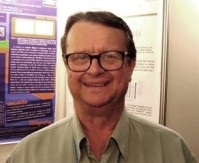
\includegraphics[width=0.15\textwidth]{figuras/foto-otavio-camargo}
\end{wrapfigure}

A qualidade do ambiente interessa a toda a sociedade.  A pureza do ar, da água e do solo é de fundamental importância para a sobrevivência do homem. Em muitas regiões do globo, os índices mínimos de pureza já não são mais alcançados. Muitos rios, lagos e represas tornaram-se depósito de resíduos urbanos, agrícolas e industriais, os solos vêm sendo degradados química, física e biologicamente e o ar tornou-se irrespirável.

A população,  percebeu a ameaça à sua existência e, então, vem reagindo de maneira firme contra a destruição do meio que a cerca, culminando com a ECO-92 e a Agenda 21.

Embora a definição de sustentabilidade seja ainda pouco consensual e às vezes até mesmo contraditória, prejudicando a definição de uma estratégia para um desenvolvimento sustentável, parece-me que, mesmo intuitivamente pensando, é o caminho que temos escolhido nas últimas décadas do 2$^\circ$ milênio.

É assim que me permito uma primeira reflexão apoiada na de Girt e que acho muito oportuna e que fosse embutida e considerada nas discussões onde se fala em desenvolvimento sustentável onde é preciso reconciliar aspectos econômicos e sociais com as dimensões biofísicas referentes aos recursos naturais e à própria capacidade dos distintos ecossistemas em responder à demanda que lhes submetam as sociedades humanas. 

O uso inadequado do solo é fonte muito importante de poluição. O descuido do homem em controlar a erosão, por exemplo, faz do solo uma fonte potencial de contaminação de correntezas e lagos, isso sem contar a sua própria perda.

O manejo inadequado de defensivos, águas de irrigação de baixa qualidade, a disposição indisciplinada de resíduos da agricultura, indústria e cidades podem redundar no acúmulo de substâncias no solo que podem ser tóxicas às plantas e, se entrarem na cadeia alimentar, podem ser letais aos animais e ao homem.

Devido a estas relações e dada sua importância no ecossistema, o solo ocupa papel de destaque no controle da qualidade do ambiente. Se esse controle vai ser de boa ou má qualidade dependerá muito da maneira como serão manejadas as reservas edáficas.

Entretanto, deve-se ter em conta em nossas discussões, mesmo que puramente técnicas, que a degradação destes recursos não é consequência inevitável do progresso humano e mesmo da densidade das populações, mas consequência de um tipo de crescimento econômico cruelmente insustentável em termos ecológicos, e desigual e injusto em termos sociais. É bom que se perceba que a degradação ambiental não é consequência do desenvolvimento, mas de uma modalidade particular deste, fazendo-se assim necessária e urgente uma correção significativa de rota.

A solução não estará então em desacelerar o desenvolvimento, mas mudar qualitativa e quantitativamente o modelo, mantendo como alvo primacial o melhoramento da qualidade de vida, porém nem sempre pensando o crescimento como aumento da produção.

Para tanto não podemos ter um Estado pequeno, fragmentado e frágil, como vemos acontecer em muitas partes do globo atualmente, mas um Estado, se pequeno, sadio e robusto, para evitar a palavra forte. A visível deterioração das instituições  públicas nos últimos anos com a difusão da ideia de enxugamento da máquina como parte do processo de modernização administrativa é um caminho muito negativo se não forem definidas urgentemente as funções que o Estado deve desempenhar na promoção de um desenvolvimento sustentável.

Explico, é consenso que um zoneamento agroecológico e o planejamento do uso da terra são ingredientes primordiais para qualquer definição de estratégia de desenvolvimento sustentável a ser adotada. Portanto, parece-me ter cabimento a pergunta: pode-se esperar sucesso de qualquer modelo nesse sentido diante de um Estado debilitado?

O momento é de muita reflexão e me resta pensar que o homem só conservará sua saúde biológica e mental se aprender a criar um ambiente sadio.

E gostaria de terminar essas poucas e rápidas reflexões com a observação feita pelo escritor Henry Thoreau: ``de que vale uma casa quando não se tem um planeta tolerável onde colocá-la?''

\address{Otávio Antonio de Camargo\\
  Instituto Agronômico de Campinas, IAC\\
  \url{http://lattes.cnpq.br/1337171805613486}\\
  \email{ocamargo@iac.sp.gov.br}}
%%% Local Variables: 
%%% mode: latex
%%% TeX-master: 4th-edition.tex
%%% End: 
\end{article}
 \newpage
\begin{article}
   \title{As ``outras'' revistas científicas}
\author{por Vidal Barrón}
\maketitle
\begin{wrapfigure}{l}{0.15\textwidth}
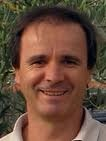
\includegraphics[width=0.15\textwidth]{figuras/foto-vidal-barron}
\end{wrapfigure}

Em 1887 a revista \href{http://www.ajsonline.org/}{\textit{American Journal of Science}}, a mais antiga dos Estados Unidos, publicou um artigo intitulado ``\textit{On the Relative Motion of the Earth and the Luminiferous Ether}''. Nesse trabalho, não foi encontrada nenhuma relação entre o movimento relativo da Terra e o suposto ``éter luminoso''. O mesmo autor desse trabalho, Albert A. Michelson, recebeu em 1907 o Prêmio Nobel de Física, pelo desenvolvimento do interferômetro, aparelho utilizado para efetuar medidas de ângulos e distâncias aproveitando a interferência de ondas electromagnéticas.

Provavelmente muitas de nossas experiências fracassadas ou negativas nunca chegaram à relevância do trabalho de Michelson. No entanto, em muitos campos da ciência a publicação de resultados inesperados podem ser de grande importância, não só porque evita que erros sejam cometidos novamente resultando em desperdício econômico, mas em alguns casos, porque ajuda a negar ideias ou hipóteses, e a criar novas.

A meta-análise, estudos que utilizam técnicas estatísticas para combinar resultados independentes sobre investigação em áreas como medicina, farmácia, biologia ou agronomia são tendenciosos. A pressão por parte das agencias financiadoras, e até mesmo a autocensura, leva muitos pesquisadores a não publicarem resultados negativos ou melhor, publicarem em revistas de baixo impacto. 

A fim de superar essas falhas da ``máquina científica'', nasceram várias revistas que coletam estes resultados inesperados, frustrantes ou negativos. Abrangendo diversas áreas do conhecimento científico, como química, física, biologia ou nanotecnologia, desde 2010 existe a \href{http://www.arjournals.com/ojs/}{\textit{The All Results Journals}}, uma revista de acesso aberto, ou seja, nem os leitores nem os autores têm que pagar para ler e/ou publicar seus artigos. Outras revistas como \href{http://www.jnrbm.com/}{\textit{Journal of Negative Results in BioMedicine}} e \href{http://www.pnrjournal.com/}{\textit{Journal of Pharmaceutical Negative Results}} também seguem essa filosofia de publicação de resultados inesperados. Muitas outras áreas, por exemplo, agronomia também poderiam se beneficiar de uma plataforma para a publicação e discussão de resultados inesperados, polêmicos, provocativos e/ou negativos.

E se os nossos resultados, embora gerados com o rigor científico necessário, também tivessem um toque de humor inesperado ou previsto? \href{http://www.jir.com/index.html}{\textit{The Journal of Irreproducible Results}} oferece a possibilidade de publicar todos os tipos de piadas, paródias, sátira e humor gráfico de caráter científico. Com mentalidade parecida, porém com maior índice de impacto, existe a \href{http://www.improbable.com/}{\textit{Annals of Improbable Research}}, editada pela prestigiada Universidade de Harvard. Esta revista  também é conhecida pelo famoso Prêmio \href{http://www.improbable.com/ig/winners/}{\textit{IgNobel}}, dado para a descoberta científica mais estranha do ano em diferentes campos da ciência. Alguns ganhadores do \textit{IgNobel} foram: Len Fisher em 1999, por sua pesquisa sobre a física de como molhar um biscoito. Lendo sua pesquisa, agora convertido em um livro \textit{best-seller}, nos inspirou no passado, a interpretar o comportamento de alguns solos brasileiros. Outro conhecido ganhador do \textit{IgNobel} foi o pesquisador Andre Geim, ganhador do Prêmio Nobel de Física em 2010 por suas pesquisas sobre o grafeno. Geim, recebeu em 2000 o \textit{IgNobel} pelo seu estudo sobre a levitação de rãs em um campo magnético. Parece, que este tipo de publicação pode ser o prelúdio de conquistas cientificas maiores!

\address{Vidal Barrón\\
  Universidade de Córdoba, UCO, Espanha\\
  \url{http://www.researchgate.net/profile/Vidal\_Barron}\\
  \email{cr1balov@uco.es}}
%%% Local Variables: 
%%% mode: latex
%%% TeX-master: 4th-edition.tex
%%% End: 
\end{article}
\newpage
\begin{article}
   \title{Eventos}
\maketitle


\section{INTERGEO}
\subsection{Istambul, Turquia, 28-29/4/2014}
O congresso é organizado pela German Society of Geodesy, Geoinformation and Land Management (DVW). 
Maiores informações podem ser encontradas no endereço \url{http://www.intergeo-eurasia.net/en/index.html}.


\section{Conferência e Feira de Geomática e Soluções Geoespaciais}
\subsection{São Paulo, Brasil, 7-9/5/2014}
O evento é organizado por MundoGEO.
Maiores informações podem ser encontradas no endereço \url{http://mundogeoconnect.com/2014/}.


\section{ISRIC'S Spring School 2014}
\subsection{Wageningen, Holanda, 12-16/5/2014}
O evento é organizado pelo International Soil Reference and Information Centre - ISRIC. Serão abordados temas relacionados ao Mapeamento Digital de Solos (MDS) e uso de softwares para análise de dados de solos.
Maiores informações podem ser encontradas no endereço \url{http://www.isric.org/content/isrics-spring-school-2014}.


\section{20th Word Congress of Soil Science}
\subsection{Jeju, Korea, 8-13/06/2014}
O congresso é organizado pela International Union of Soil Sciences (IUSS). 
Maiores informações podem ser encontradas no endereço \url{http://www.20wcss.org/}.


\section{12th International Conference of Precision Agriculture}
\subsection{Sacramento, Califórnia (USA), 20-23/07/2014}
O congresso é organizado pela Sociedade Internacional de Agricultura de Precisão.
Maiores informações podem ser encontradas no endereço \url{https://www.ispag.org/ICPA/}.


\section{XX Congresso Latinoamericano de la Ciencia Del Suelo}
\subsection{Cusco, Perú, 9-15/11/2014}
O evento é organizado pela Sociedade Latinoamericana de Ciência do Solo (SLCS).
Maiores informações podem ser encontradas no endereço \url{http://www.xxcongresolatinoamericanodesuelosperu.org/programa.php}.


\section{6th Global Workshop on Digital Soil Mapping}
\subsection{Nanjing, China, 11-14/11/2014}
O evento é  organizado pelo Instituto de Ciência do Solo da Academia Chinesa de Ciências. O prazo para submissão de trabalhos é 31/07/2014.
Maiores inforamçoes podem ser encontradas no endereço \url{http://dsm2014.csp.escience.cn/}.


\address{Jean Michel Moura-Bueno\\
    Universidade Federal de Santa Maria\\
    \email{bueno.jean1@gmail.com}}
\end{article}
\newpage
\begin{article}
   \title{Pedometria na SBCS}
\maketitle
\newcommand{\estrutura}{\href{http://www.sbcs.org.br/a-sbcs/estatuto/}{estrutura científica}}
\newcommand{\SBCS}{\href{http://www.sbcs.org.br/}{SBCS}}
\newcommand{\IUSS}{\href{http://www.iuss.org/}{IUSS}}
\newcommand{\boletim}{\href{http://www.iuss.org/images/stories/IUSS\%20Bulletin\%201\%20-\%20117/00000097.pdf}{Boletim 97}}
\newcommand{\EspacoTempo}{\href{http://www.sbcs.org.br/comissoes-especializadas/divisao-1-solo-no-espaco-e-no-tempo/}{Espaço e no Tempo}}
\newcommand{\PedometronOnze}{\href{http://www.pedometrics.org/Pedometron/pedometron11.pdf}{Pedometron 11}}
\newcommand{\PedometronDoze}{\href{http://www.pedometrics.org/Pedometron/pedometron12.pdf}{Pedometron 12}}

A atual \estrutura{} da Sociedade Brasileira de Ciência do Solo (\SBCS) foi definida na Assembleia Geral dos Congressos Brasileiros de Ciência do Solo realizados em Fortaleza (2009) e Uberlândia (2011). Na época, o objetivo principal foi adequar-se a estrutura científica da União Internacional de Ciência do Solo (\IUSS), a qual fora definida no Congresso Mundial de Ciência do Solo realizado na Tailândia em 2002. Tal estrutura inclui Divisões, Comissões, Grupos de Trabalho, e Comitês Permanentes (\boletim). São as Divisões, as Comissões e os Grupos de Trabalho os responsáveis por desenvolver as atividades científicas da SBCS e da IUSS.

Hoje são quatro as Divisões da SBCS e da IUSS, cada uma subdividida em Comissões. A Divisão I da SBCS, chamada Solo no \EspacoTempo, possui três Comissões: Gênese e Morfologia do Solo, Levantamento e Classificação do Solo, e Pedometria.

A coordenação da Divisão I é a seguinte:

\begin{itemize}
 \item Diretor: Lúcia Helena Cunha dos Anjos - UFRRJ
 \item Vice-diretor: Humberto Gonçalves dos Santos - EMBRAPA
 \item Membro titular: Elpídio Inácio Fernandes Filho - UFV
 \item Membro suplente: Cristiane Valéria de Oliveira - UFMG
\end{itemize}

\subsection{Comissão de Pedometria}

A Comissão de Pedometria da IUSS foi criada no Congresso Mundial de Ciência do Solo realizado na Tailândia em 2002 a partir do Grupo de Trabalho em Pedometria, um dos mais ativos na época. Muitas foram as discussões sobre a Divisão a qual a Comissão de Pedometria deveria pertencer (\PedometronOnze{} e \PedometronDoze). Isso porque a pedometria constitui um campo que abrange muitos outros campos da ciência do solo, como estatística, matemática, física, química, informática, biologia, mineralogia, geografia \textit{et cetera}. Apesar da multitude de campos de atuação, a nova estrutura científica da IUSS exige que as Comissões façam parte de uma única Divisão. Como a maior parte das contribuições da pedometria estão relacionadas à variabilidade espaço-temporal das propriedades do solo, o consenso foi de que a Divisão I seria a mais apropriada.

A Comissão de Pedometria da SBCS possui em seu escopo os seguintes temas:

\begin{itemize}
 \item Fotointerpretação e sensoriamento remoto
 \item Mapeamento digital de solos
 \item Variabilidade espacial e temporal de atributos de solo (geoestatítica)
 \item Análise espectral (refletância)
 \item Processamento de dados de solos
\end{itemize}

A coordenação da Comissão de Pedometria é a seguinte:

\begin{itemize}
 \item Coordenador: Maria de Lourdes Mendonça Santos - EMBRAPA
 \item Vice-coordenador: Elpídio Inácio Fernandes Filho - UFV
 \item Membros titulares: César da Silva Chagas - EMBRAPA, e José Alexandre Melo Demattê - ESALQ/USP
 \item Membros suplentes: Gustavo de Mattos Vasques - EMBRAPA, e Ricardo Simão Diniz Dalmolin - UFSM
\end{itemize}

\subsection{Grupo de Trabalho em Mapeamento Digital de Solos}

Os Grupos de Trabalho são grupos científicos criados em caráter temporário para tratar de problemas específicos da ciência do solo. Atualmente a IUSS possui 17 Grupos de Trabalho atuando nos mais diversos temas.

O primeiro Grupo de Trabalho da SBCS foi criado durante o Congresso Brasileiro de Ciência do Solo realizado em Florianópolis (2013). Trata-se do Grupo de Trabalho em Mapeamento Digital de Solos (GT-MDS). A solicitação foi feita pela Rede Brasileira de Pesquisa em Mapeamento Digital de Solos (RedeMDS), constituída por pesquisadores de diversas instituições de ensino e pesquisa brasileiras.

O GT-MDS possui como missão elaborar projetos de ação conjunta e integrada para o mapeamento digital dos solos do Brasil e gerar sinergia entre os pesquisadores brasileiros para promover o avanço da pesquisa em mapeamento digital de solos.

Especificamente, o GT-MDS possui como objetivos:

\begin{itemize}
 \item Consolidar a Rede Brasileira de Mapeamento Digital de Solos do Brasil
 \item Realizar o mapeamento digital de atributos do solo em todo o território brasileiro
 \item Realizar o mapeamento digital de classes de solos
 \item Propor metodologia e validação de mapeamento digital de classes e/ou atributos de solos em áreas pilotos do território brasileiro
 \item Realizar treinamento em mapeamento digital de solos
\end{itemize}

A fim de cumprir sua missão e alcançar seus objetivos, o GT-MDS procura realizar encontros anuais. Estes encontros geralmente ocorrem concomitantes a outros eventos de abrangência nacional a fim de estimular a interdisciplinaridade e otimizar os recursos disponíveis. Nos anos em que é realizado o Congresso Brasileiro de Ciência do Solo, o GT-MDS reúne-se para avaliar as atividades científicas passadas, definir as atividades científicas futuras, e faz um relato das mesmas ao Coordenador Geral da Divisão I.

A coordenação atual do GT-MDS é composta pelos seguintes pesquisadores:

\begin{itemize}
 \item Coordenador geral: Márcio Francelino - UFV
 \item Coordenador Regional I: Ricardo Simão Diniz Dalmolin - UFSM
 \item Coordenador Regional II: José Alexandre M. Demattê - ESALQ/USP
 \item Coordenador Regional III: Elpidio Inácio Fernandes Filho - UFV
 \item Coordenador Regional IV: Gustavo de Mattos Vasques - EMBRAPA SOLOS
 \item Coordenador Regional V: Gustavo Souza Valladares - UFPI
\end{itemize}
%%% Local Variables: 
%%% mode: latex
%%% TeX-master: 5th-edition.tex
%%% End:
\end{article}
\newpage
\begin{article}
   \title{Instruções aos autores}
\maketitle
\newcommand{\SBCS}{\href{http://www.sbcs.org.br/}{SBCS}}
\newcommand{\Nature}{\href{http://www.nature.com/nature/authors/gta/}{Nature}}
\newcommand{\Science}{\href{http://www.sciencemag.org/about/authors}{Science}}
\newcommand{\CreativeCommons}{\href{http://creativecommons.org/licenses/by-sa/2.0/}{CC-BY-SA}}
\newcommand{\Kile}{\href{http://kile.sourceforge.net/}{Kile}}
\newcommand{\MiKTeX}{\href{http://miktex.org/}{MiKTeX}}
\newcommand{\aquiLaTeX}{\href{https://docs.google.com/document/d/1F3IXzWNCeUrwKeFxA4iHS3aw1nforK1IqB126xbawvA/edit?usp=sharing}{aqui}}
\newcommand{\aquiWord}{\href{https://docs.google.com/document/d/1pyK03RBDPhOMrTVfvj9NcEfjGWeswqYbYDqEKq83drQ/edit?usp=sharing}{aqui}}
\newcommand{\Geoderma}{\href{http://www.elsevier.com/author-schemas/latex-instructions}{Geoderma}}
\newcommand{\EJSS}{\href{http://onlinelibrary.wiley.com/journal/10.1111/\%28ISSN\%291365-2389/homepage/ForAuthors.html}{European Journal of Soil Science}}

\subsection{Escopo e política}

\pedometria{} é a \textit{Newsletter} (boletim técnico-científico) da Comissão de Pedometria da Sociedade Brasileira de Ciência do Solo (\SBCS). Assim sendo, dedica-se à publicação de artigos relacionados à aplicação de métodos matemáticos e estatísticos para o estudo da gênese e distribuição dos solos, o que abrange desde discussões conceituais até a aplicação prática de sensores e modelos. Especificamente, os seguintes tópicos costumam ser cobertos:

\begin{itemize}
 \item explicitação de conceitos pedométricos;
 \item entrevista com pedometrista;
 \item opinião sobre tema pedométrico relevante;
 \item descrição de equipamentos e sensores remotos;
 \item descrição de softwares e suas funcionalidades;
 \item eventos técnico-científicos;
 \item expressão artística em pedometria;
 \item novas publicações científicas em pedometria.
\end{itemize}

Os artigos submetidos para publicação em \pedometria{} NÃO DEVEM ser formais como aqueles geralmente submetidos para revistas científicas tradicionais da área de pedometria. DEVE-SE usar linguagem CLARA e INFORMAL, preferencialmente na VOZ ATIVA. O uso da voz ativa é uma recomendação para publicação em ambas as revistas \Nature{} e \Science:

\begin{description}
 \item \textit{Nature} ``Nature journals like authors to write in the active voice (`we performed the experiment...') as experience has shown that readers find concepts and results to be conveyed more clearly if written directly.''
 \item \textit{Science} ``Use active voice when suitable, particularly when necessary for correct syntax (e.g., `To address this possibility, we constructed a lZap library ...,' not `To address this possibility, a lZap library was constructed...').''
\end{description}

Conceitos pedométricos devem ser introduzidos com SENSIBILIDADE, tendo em mente que os leitores podem os desconhecer e/ou não possuir base conceitual suficiente para compreendê-los em uma única leitura. A estrutura do artigo deve ser concebida da mesma maneira que o fazemos para contar uma história a um amigo ou familiar, a fim de cativar o leitor e envolvê-lo no emocionante universo da pedometria. Caso a comissão editorial entenda que a compreensão do texto exija aprofundado conhecimento prévio do leitor, os autores serão solicitados a torná-lo mais simples e amigável.

O escopo e política de \pedometria{} coloca-a como veículo de divulgação e desmistificação da pedometria no Brasil. Trata-se de uma publicação com três edições anuais que permite aos pesquisadores brasileiros divulgar suas pesquisas pedométricas e, sobretudo, conhecerem uns aos outros. Isso é importante porque, assim como a própria pedometria, a maioria dos pedometristas também são bastante jovens, muitos dos quais ainda estão desenvolvendo seus estudos de mestrado e/ou doutorado. Por este motivo, \pedometria{} é distribuída gratuitamente via Internet, estando registrada sob a licença Creative Commons Atribuição-Compartilha Igual 3.0 Não Adaptada (\CreativeCommons).\\
\\
\begin{figure}[h!]
 \centering
 
\includegraphics[width=0.8\textwidth]{figuras/cc-by-sa}
 \caption{Licença Creative Commons Atribuição-Compartilha Igual 3.0 Não Adaptada.}
\end{figure}

\subsection{Estrutura do artigo}

A estrutura do artigo é inteiramente definida pelo(s) autor(es). Sugere-se que sejam utilizadas subdivisões em até dois níveis de profundidade (seções e subseções), não necessariamente definidas como em artigos científicos tradicionais. Os artigos podem ter, além do título, um subtítulo. Resumo e palavras-chave não são utilizados.

\subsubsection{Figuras e tabelas}

Figuras e tabelas são recomendadas, sendo uma foto do(s) autor(es) obrigatória. Figuras devem ser preparadas no formato PNG, com resolução mínima de 300 dpi.

\subsubsection{Referências bibliográficas}

Referências bibliográficas não são mandatórias, sobretudo no caso de artigos apresentando a opinião do autor sobre um tema pedométrico. Caso citações sejam feitas ao longo do texto, a lista de referências deve ser organizada na ordem em que as citações são feitas no texto. Importante notar que o estilo de citação numérica sobrescrita da \textit{Nature} é utilizado.

A lista de referências bibliográficas deve conter até cinquenta itens. O conteúdo da lista de referências deve ser econômico, incluindo apenas informações fundamentais para a sua identificação. Artigos, trabalhos em anais de eventos ou em coleções, e trabalhos publicados em veículos periódicos similares, devem ser formatados da seguinte maneira:

\vspace{0.5cm}
\noindent{A.B. McBratney, M.L. Mendonça-Santos, B. Minasny (2003) On digital soil mapping. \textit{Geoderma}, 117:3-52. \doi{10.1016/S0016-7061(03)00223-4}}
\vspace{0.5cm}

\noindent{onde \textit{link} refere-se ao endereço na Internet onde o referido documento pode ser encontrado. No caso de artigos científicos recomenda-se utilizar o Digital Object Identifier (\href{http://www.doi.org/}{DOI}). Livros, teses, dissertações, relatórios e outros meios de publicação não periódicos devem ser formatados da seguinte maneira:}

\vspace{0.5cm}
\noindent{H. Jenny (1994) \textit{Factors of soil formation - a system of quantitative pedology}. Toronto: Dover Publications.}
\vspace{0.5cm}

\noindent{Caso as publicações não periódicas estejam disponíveis na Internet, um link deve ser adicionado assim como para as publicações periódicas.}

\subsection{Preparo do artigo}

Os artigos podem ser preparados utilizando processadores de texto tradicionais, como por exemplo o MS Office Word (*.doc) e o LibreOffice Writer (*.odt), ou a linguagem de marcação \LaTeX() (*.tex). Preferência deve ser dada ao formato \LaTeX() sempre que possível a fim de facilitar o trabalho da equipe editorial. Documentos no formato PDF não são aceitos.

\subsubsection{Word ou Writer}

Um modelo para preparo do artigo usando processadores de texto tradicionais pode ser acessado clicando \aquiWord.

\subsubsection{\LaTeX}

\href{http://pt.wikipedia.org/wiki/Latex}{\LaTeX} é uma \href{http://pt.wikipedia.org/wiki/Linguagem_de_marca\%C3\%A7\%C3\%A3o}{linguagem de marcação} amplamente utilizada para a produção de textos matemáticos e científicos devido à sua alta qualidade tipográfica. Utilizar uma linguagem de marcação para elaboração de textos constitui no uso de comandos escritos para definir a formatação do documento, ao contrário dos editores tradicionais que oferecem abas e caixas de diálogo para clicar e definir parâmetros de formatação. Na prática, ao produzir um texto em \LaTeX, o autor não vê o produto final formatado na tela do computador imediatamente, mas apenas o texto e os comandos de formatação. O objetivo é distanciar o autor o máximo possível da apresentação visual do artigo, ou seja, ao invés de trabalhar com ideias visuais, o autor é encorajado a trabalhar com conceitos lógicos independentes da apresentação final do artigo. Além disso, linguagens de marcação como o \LaTeX{} permitem agilizar a confecção do documento final (PDF) e reproduzir o conteúdo em outros formatos para apresentação em meio digital como o html. Atualmente, importantes revistas científicas da área de pedometria adotam o \LaTeX{} para a confecção de seus artigos, como por exemplo \Geoderma{} e \EJSS.

Apesar de diferente dos processadores de texto tradicionais, usar \LaTeX{} é bastante fácil, sendo necessário apenas compreender a sua lógica de funcionamento. Para isso é bom dar uma olhada no \href{http://www.stdout.org/~winston/latex/}{Manual Rápido \LaTeX{}} para conhecer alguns comandos básicos. O preparo dos artigos usando \LaTeX{} pode ser feito usando softwares como Bloco de Notas, WordPad, e Gedit. Entretanto, é mais aconselhado usar um software específico para a edição de documentos em \LaTeX, como o \Kile{} e o \MiKTeX. Tais softwares auxiliam a inserção dos comandos necessários para a formatação do texto sem a necessidade de memorizá-los.

Um modelo para preparo do artigo usando \LaTeX{} pode ser acessado clicando \aquiLaTeX.

\subsection{Submissão}

Qualquer pessoa pode submeter um artigo para publicação em \pedometria{} sem qualquer custo. Quando o artigo estiver pronto, adicione todos os arquivos utilizados (inclusive as figuras originais) à uma pasta comprimida e envie para a comissão editorial usando o endereço de e-mail \email{pedometria.news@gmail.com}.

\subsection{Comissão editorial}

Alessandro Samuel-Rosa\\
\textit{ISRIC - World Soil Information}\\
\textit{Wageningen University and Research Center}\\
\email{alessandro.rosa@wur.nl}\\
\\
André Geraldo de Lima Moraes\\
\textit{Curso de Pós-Graduação em Agronomia-Ciência do Solo}\\
\textit{Universidade Federal Rural do Rio de Janeiro}\\
\email{andrehmuz@hotmail.com}\\
\\
Diego Silva Siqueira\\
\textit{Grupo de Pesquisa Caracterização do Solo para fins de Manejo Específico}\\
\textit{Universidade Estadual Paulista - Campus Jaboticabal}\\
\email{diego\_silvasiqueira@yahoo.com.br}\\
\\
Jean Michel Moura-Bueno\\
\textit{Programa de Pós-Graduação em Ciência do Solo}\\
\textit{Universidade Federal de Santa Maria}\\
\email{bueno.jean1@gmail.com}

\subsection{Observação}

Iniciamos tratativas com a Sociedade Brasileira de Ciência do Solo para que toda a sua documentação e números publicados de \pedometria{} fiquem hospedados no \textit{website} \url{http://www.sbcs.org.br}. Infelizmente a Sociedade  Brasileira de Ciência do Solo não possui infraestrutura disponível para que isso seja possível. Enquanto isso, \pedometria{} fica temporariamente hospedada no \textit{website} \url{https://sites.google.com/site/pedometria/}, impedindo a obtenção de ISSN.

\subsection{Agradecimento}

Gostaríamos de agradecer o conselho editorial do \href{http://grass.osgeo.org/newsletter/}{GRASS News} do projeto GRASS pois, sem a sua contribuição com os arquivos *.tex e *.sty do GRASS News, \pedometria{} teria levado muito mais tempo para atingir o nível atual.
%%% Local Variables: 
%%% mode: latex
%%% TeX-master: 4rd-edition.tex
%%% End:
\end{article}
\end{document}
%%% Local Variables: 
%%% mode: latex
%%% TeX-master: 4rd-edition.tex
%%% End: 